\documentclass[12pt]{article}
\usepackage{amsmath}
\usepackage{amssymb}  
\usepackage{hyperref}
\usepackage[pdftex]{color,graphicx}

\oddsidemargin -0.04cm \evensidemargin -0.04cm \setlength{\topmargin}{-0.5in} \textwidth 16.59cm \textheight 23cm
\newcommand{\vanish}[1]{}

\begin{document}
\thispagestyle{empty}
\begin{center}
\huge\bf {\bf GemIdent} 1.0 User Manual
\end{center}

\vspace{3cm}
\begin{figure}[htp]
\centering
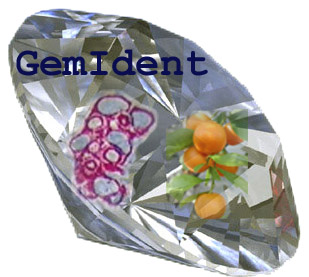
\includegraphics[width=154pt,height=139pt]{logo.jpg}
\label{fig:logo}
\end{figure}


\vspace{6cm}
\begin{flushright} 

\vspace{1cm}
\sf
Adam Kapelner \\
Susan Holmes \\
Peter P. Lee \\
\vspace{1cm}
{\tt www.GemIdent.net} \\
\vspace{1cm}
{\footnotesize \copyright 2007 The Board of Trustees of the Leland Stanford Junior University. All Rights Reserved.}
\end{flushright}

\pagebreak

\section{Introduction\label{Introduction}}

{\bf GemIdent} is a revolutionary program that identifies objects of interest in images. The engine leverages modern artificial intelligence algorithms and takes advantage of color information. {\bf GemIdent} works optimally when objects of interest look alike and the images only have a few relevant colors.

\section{Getting Started\label{getting_started}}

\subsection{Downloading and Installing}

Head to {\tt www.gemident.net/download.html}, agree to the license and fill out the form. You will then be provided with a download link. Unzip the contents to a folder on your hard drive.

\subsection{Running GemIdent}

GemIdent requires Java 6 and at least 512MB of memory. You can download the latest Java Runtime Environment (JRE) at {\tt www.java.com/en/download/}

If you are using Windows, the zip file already contains a launch file. Double click the ``GemIdent'' shortcut to begin. If you are not using Windows, create a script file in the unzipped directory with the following line: {\tt java -jar gemIdent.jar -Xmx500m -Xss5m} Make sure Java is in your system path, and execute the script.

\subsection{Beginning a new project\label{new}}

Place only those image files you wish to identify into one directory. If your images represent subimages in the context of a larger global image, currently {\bf GemIdent} will only be able to examine the global data if the images were taken with the Bliss Slide Scanner (Bacus Laboratories, Inc), the NanoZoomer (Bacus Laboratories, Inc) or the Nuance Multispectral Imaging System (CRI, Inc). Ensure that the initialization file from the scanner is in the directory and image files not part of the high resolution scan are {\emph{not}} in the directory. Support for other systems will be added soon.

Start {\bf GemIdent} and click on the \framebox{\sf new} button (the page icon). Enter the name of the new analysis under the field {\sf Project Name.} Then use the directory chooser ``\framebox{\sf  ...}'' button to locate the {\emph{directory}} of the image set. Next choose the type of image set and press \framebox{\sf  Okay} to generate the new project.

\subsection{Saving a project}

When you wish to save, use the {\sf  Save Project} menu item in the {\sf File} menu or press {\tt CTRL+S}. This command will generate `{\tt <project>.gem}' in the directory of the image set where {\tt <project>} is the name of the analysis. The proprietary file format, {\tt gem}, is just an {\tt XML} dump of the training data and the user's preferences and can be edited with any text editor.

\subsection{Opening a saved project\label{open}}

Start {\bf GemIdent} and click the \framebox{\sf  open} button (the folder icon). Use the file chooser to find the project's {\tt .gem} file. If you are already in another analysis you can use the \framebox{\sf  Open Project} item in the {\sf File} menu or {\tt CTRL+O}.

\section{Training\label{training}}

{\bf GemIdent} uses statistical supervised-machine learning algorithms in order to perform automated identification of the images. This involves some work on the part of the user to manually identify both the colors of interest as well as examples of the sought objects themselves.

Training is, at the minimum, a two-stage process - color selection (via the {\sf  Color Selection} panel) and phenotype training (via the {\sf  Phenotype Training} or {\sf  Phenotype Retraining} panel). 

\subsection{Color Selection\label{color_selection}}

The goal of color selection is to identify each of the relevant colors in the image set. In the example of histology, if all nuclei are counterstained blue, antigen A was stained using red, antigen B was stained using brown, and the background intercellular matrix is white-gray, that would be four relevant colors. When finding oranges in an orange tree, the oranges are orange and the surrounding leaves are greem, hence two relevant colors.

Color training is only necessary when the relevant colors were not previously ``filtered.'' In a histological analysis using an image set obtained from the Nuance Multispectral Imaging System, the scanner has already separated the chromagens by using special optical filters and recorded each to a separate image file. Due to this, the {\sf  Color Selection} panel has been removed for projects of this image set type.

\begin{figure}[htp]
\centering
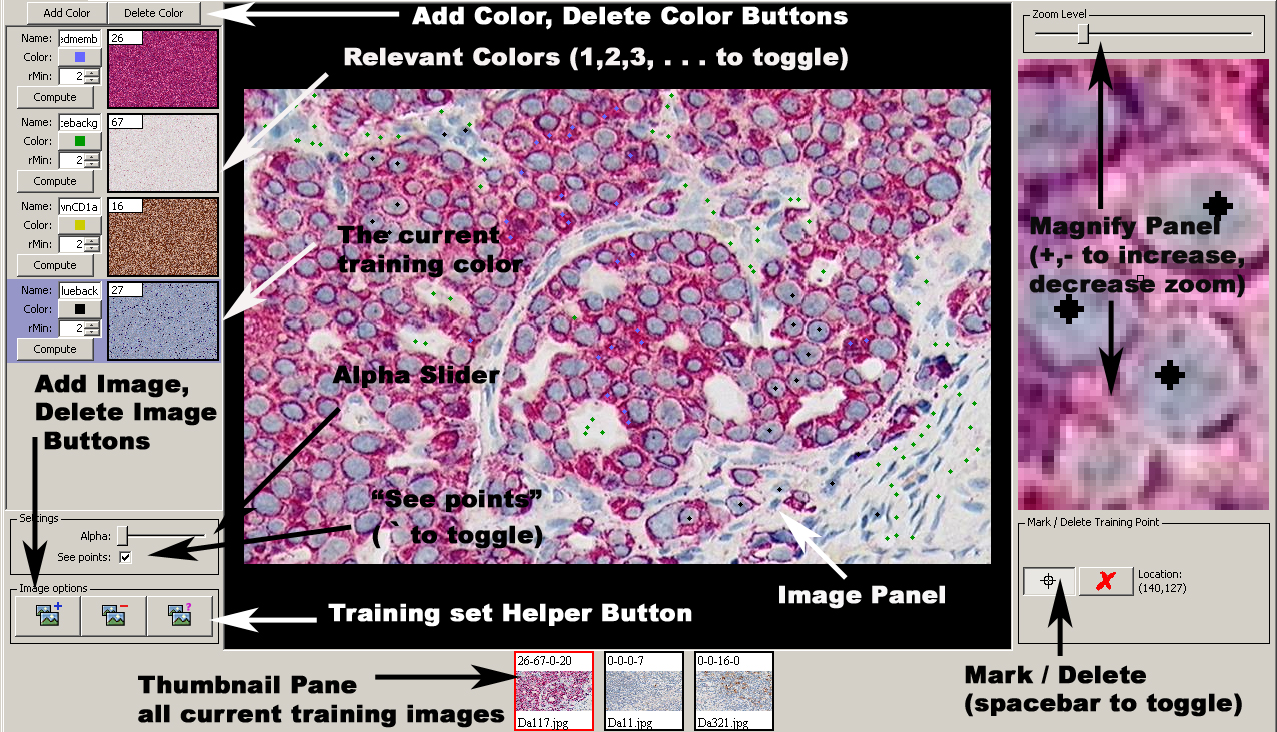
\includegraphics[width=476pt,height=281pt]{colorselection.jpg}
\label{fig:colorselection}
\caption{\sf The anatomy of the Color Selection panel including the keyboard shortcuts. The image being trained is a lymphnode from the Kohrt study\cite{kohrt}.}
\end{figure}

\subsubsection{Establishing Colors}

Begin by clicking the \framebox{\sf Add Color} button and typing a short identification name
of your choice (eg ``red''). Repeat for all colors. If at any time you wish to remove a color, click the \framebox{\sf  Delete Color} and select the color to be removed. 

\subsubsection{Adding Images and Using the Training Helper}

Click the \framebox{\sf  Add Image} button and select an image that has a good representation of one or more of the relevant colors. A thumbnail for that image will be placed on the bottom of the window in the rectangle known as the ``thumbnail pane.''

If the image set is from a Bliss or NanoZoomer, click the \framebox{\sf  Training Helper} button to bring up a webpage of the entire scan. Pick a size appropriate to the scan. Mousing over any part of the image will reveal the filename. Clicking anywhere on the scan will link to that image. From here, you can get a good idea of which images contain good examples of the relevant colors.

If at any time you wish to remove a training image, click the \framebox{\sf  Delete Image} button and select the filename of the image.

\subsubsection{Entering examples}

Select the relevant color you want to train on the left panel. The subpanel should now be highlighted. Click on a location in the image that expresses this color. Use the magnifying window to help ensure the selection point is exact. Upon clicking you will notice the icon within the subpanel will change color reflecting the colors you've selected. The number label will also increase by one, keeping track of your total number of training points for this color. Also, the thumbnail of the example image you're training will show an updated count of the training points within that specific image.

The {\sf color} option allows you to specify the color of your training points. This is purely an aesthetic tool. It is recommended to choose a color with good contrast against the relevant color being trained so you can easily see your training points.

The {\sf rMin} option allows you to specify the impact radius of your clicks. All points within that radius will be included in the training set for that color. The minimum {\sf rMin} is zero (meaning the sole pixel specified) and the maximum {\sf rMin} is three (the pixel specified plus the 28 surrounding pixels).

If at any time a mistake is made, click the \framebox{\sf  X} button in the ``Mark / Delete'' frame and then click over the point to delete it. You can toggle conveniently between mark and delete by using the {\tt spacebar}.

If you wish to toggle your training points on or off, click the \framebox{\sf  See points} checkbox. This may be useful if there are hundreds of training points and the underlying image can no longer be seen.

Although picking a good color contrast is necessary, the training points may still be hard to discern from the underlying image (this is especially relevant when {\sf rMin} is set to zero). In this case, use the \framebox{\sf  Alpha} slider which will create a circle mask with varying opacity around each of the training points.

\begin{figure}[htp]
\centering
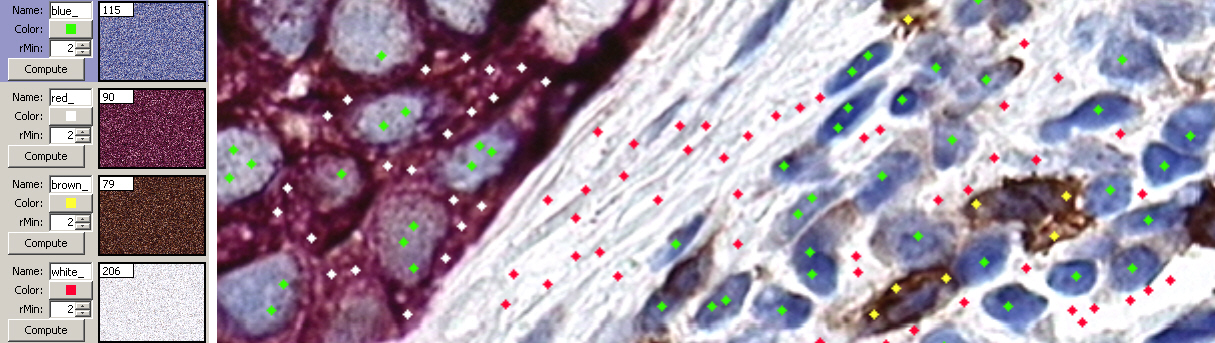
\includegraphics[width=476pt,height=135pt]{colorexamples.jpg}
\label{fig:colorexamples}
\caption{\sf An example of color selection in an immunohistochemically stained lymphnode from the Kohrt study\cite{kohrt}. The red is Fast Red marking AE1/AE3, the brown is DAB marking CD4, and the blue is a background nuclear conterstain. The left is a screenshot showing the four established colors and the right is a highly-magnified snippet of a training image, with all four colors properly trained by the user.}
\end{figure}

\subsubsection{Computation}

When you have selected a representative training set for each of the relevant colors (with at least ten points per color), the last step is to hardwire the color distribution into {\bf GemIdent}, this is done by standardizing and normalizing the multivariate colors using the Mahalonobis transform. Click the\framebox{\sf Compute} button within each of the relevant color's subpanel. This step is obligatory for {\bf GemIdent} to function during the later classification and if skipped, you will be prompted later. A 32MB file with no extension is now saved in the {\tt colors} subdirectory with the name of the relevant color. (Please note: if the relevant color is removed from the analysis, this file will be deleted from the hard drive).

Once the color information for a given color has been computed, point additions or deletions will not be visible to {\bf GemIdent}. If you would like to truly alter the training set, please reclick the \framebox{\sf Compute} button and press {\tt Yes} when it warns of overwriting the file.

\subsubsection{General Tips}

If the colors vary within the image, ensure your training includes examples throughout the spectrum of this distribution. However, if the colors differ substantially, it may be appropriate to ``split'' the relevant colors into two or more sub-colors. The more specific information, the better for {\bf GemIdent}, but the slower the analysis. Color splitting is at your discretion and you must experiment to find what works the best for any given application.

It is always a good idea to start using the program with images you understand well and where you can monitor the effect of your different choices. The orange grove files have been supplied for experimentation.

\subsection{Phenotype Training}

The goal of phenotype training is to identify a representative sample of each of the populations of object types sought. These different classes of objects are dubbed ``phenotypes'' because {\bf GemIdent} was originally designed to locate cell phenotypes in microscopic images. This term is used in a very general sense here to specify categories of objects we are trying to distinguish.  In the example of histology, the blue nuclei with brown membrane would be one phenotype, and the blue nuclei with a red membrane may be another phenotype. In the example of the orange tree, the oranges themselves would be the sole phenotype.

\begin{figure}[htp]
\centering
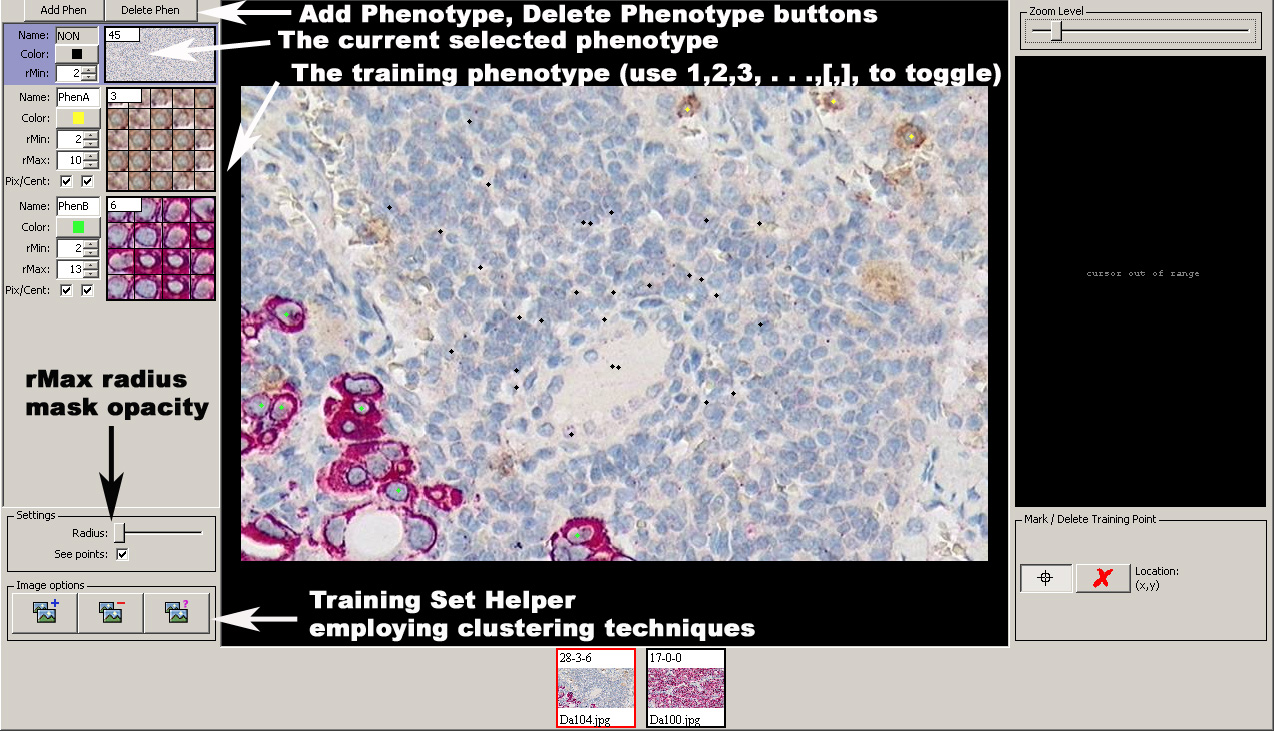
\includegraphics[width=476pt,height=281pt]{phenotypetraining.jpg}
\label{fig:phenotypetraining}
\caption{\sf The anatomy of the panel including the keyboard shortcuts. Only the differences from the {\sf color selection} panel have been labeled. The image being retrained is a lymphnode from the Kohrt study\cite{kohrt}.}
\end{figure}

\subsubsection{Establishing Phenotypes}

Begin by clicking the \framebox{\sf Add Phen} button and type a short identification name (eg ``oranges''). Repeat for all phenotypes. If at any time you wish to remove one, click the \framebox{\sf Delete Phen} and select the phenotype to be removed.

Phenotype training requires a ``NON'' phenotype which cannot be removed (see ``Entering Examples'' below).

\subsubsection{Adding and Removing Images}

To add an image to the training set, click the \framebox{\sf Add Image} button. Choose an image that has good examples of one or more phenotypes.

If at any time you wish to remove a training image, click the \framebox{\sf Delete Image} button and select the filename of the image.

\subsubsection{Using the Training Helper}

The training helper can help organize the images in the set. Click the \framebox{\sf Training Helper} button to bring up its dialog box. {\bf GemIdent} will now generate information about each image using the relevant colors from the {\sf color selection} and use it to cluster like images together. 

Select the number of clusters using the slider and click \framebox{\sf Compute}. A webpage with the separated clusters will be opened. If the image set is from a Bliss or NanoZoomer, a color-coded view of the entire scan will appear first on the webpage. Pick a size appropriate to the scan. Mousing over any part of the image will reveal the filename. Clicking anywhere on the scan will link to that image.

Since there is no color training when analyzing CRI Nuance sets, the training helper is disabled.

\subsubsection{Entering examples}

Phenotype training proceeds the same as color selection with some major differences.

You are now required to give the computer examples of what is {\emph{not}} an object of interest. This is achieved through training the ``NON'' phenotype. In the histology example (see {\tt www.GemIdent.net}), this would be the background extracellular matrix. If you are only looking for cell nuclei (in order to get accurate counts or do spatial analyses), the cell membrane would also be marked with ``NON'' (see Fig.\ref{fig:histology}) In the orange grove example (see {\tt www.GemIdent.net}), this would be the leaves, the sky, and the ground.

When selecting a point, please aim for the  geometric center of the object as this will allow a more accurate identification. The image in the subpanel becomes a matrix of examples of the phenotype. Notice that as new points are selected, the matrix will be updated. Ensure at least 15 examples are provided for each phenotype.

\begin{figure}[htp]
\centering
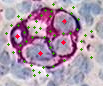
\includegraphics[width=206pt,height=168pt]{histology.jpg}
\label{fig:histology}
\caption{\sf An example of proper training --- a magnified snippet of a microscopic image of immunohistochemically stained lymph node from the Kohrt study\cite{kohrt}. The cancer cells are stained with Fast Red red marking AE1/AE3. There is a background nuclei counterstain that appears blue. The phenotype of interest are cancer cell nuclei. Training points for the phenotype appear bright red and training points for the ``NON'' appear green. The image is highly-magnified to show detail.}
\end{figure}

The {\sf rMax} option allows you to specify the maximum radius of an object. The computer will use all information within a disk of radius 150\% of this rMax 
parameter
during identification. An rMax that is too small will disallow {\bf GemIdent} from using relevant surrounding information, but an rMax too large will slow down identification. The {\sf rMax} value will determine the size of the example images in the subpanel.

The \framebox{\sf Alpha Slider} from the {\sf color selection} panel is now a \framebox{\sf Radius} slider. It has the same function, but the radius of the mask will reflect the {\sf rMax} for the given phenotype. Using the slider is a good way to ensure a proper {\sf rMax} selection.

The {\sf Pix/Cent} checkboxes allow the user to specify the appropriate type of identification. If the \framebox{\sf Cent} box (the box on the right) is checked, {\bf GemIdent} will try to locate the centroids of this phenotype when it finds them. If unchecked, {\bf GemIdent} will only identify pixels that it thinks belong to this phenotype. If the \framebox{\sf Pix} box (the box on the left) is unchecked, this phenotype will be left out of the identification completely.

\subsubsection{General Tips}

Ensure your training includes examples throughout the spectrum of this distribution. Do not neglect the ``NON'' phenotype. Make sure you give {\bf GemIdent} not only ample examples of the background, but give examples of the borders of the objects to the background as tight as possible to increase identification resolution.

If the phenotypes vary in size, ensure that you give examples of small and large objects. This will allow for more accuracy in centroid-finding. 

Again, it is a good idea to experiment with images where the phenotype choice is clearcut
so you can double check the effect of manipulating the input parameters on the software.

\section{Classification}

After both stages of training, the images are ready to be classified. Using the examples from training, {\bf GemIdent} will now create a statistical machine-learning classifier that will classify the images. 

\begin{figure}[htp]
\centering
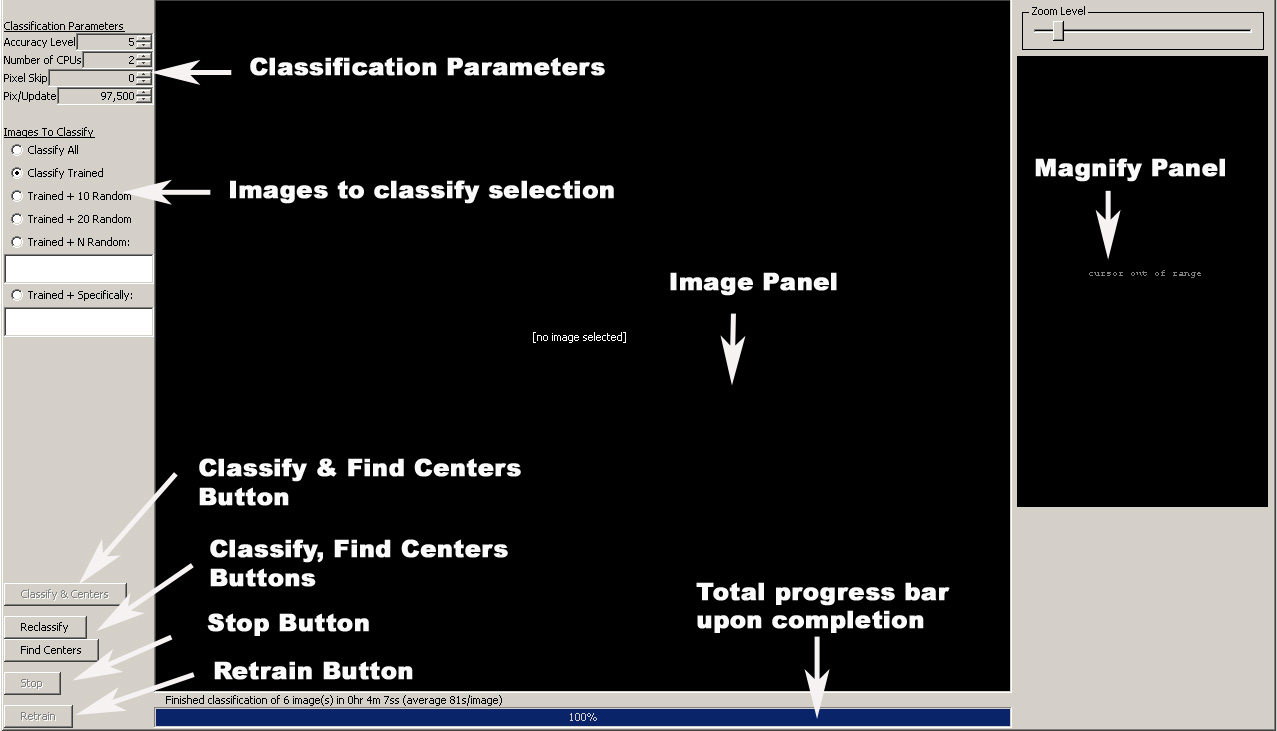
\includegraphics[width=476pt,height=281pt]{classification.jpg}
\label{fig:classification}
\caption{\sf The anatomy of the classification panel. There are no keyboard shortcuts.}
\end{figure}

\subsection{Classify}

The essential step is to ``classify'' the pixels of the target images into the classes {\em \{ ``NON,'' ``PhenA,'' ``PhenB,'' . . . \}}. Choose parameters and the images to classify and click the \framebox{\sf Classify} button.

{\bf GemIdent} will prompt if you want to delete all previous identification files as well as output files.
 
\subsubsection{Classification Parameters}

The {\sf accuracy level} option allows the user to select how accurate the classification of pixels will be. Lower levels will run faster and less accurate and higher levels, vice versa. Internally, {\bf GemIdent} employs Random Forests as its statistical learning algorithm and the {\sf accuracy level} is the number of decision trees in the forest. The minimum is five and the maximum is 250. Usually 50 provides an accurate analysis. This parameter must be experimented with and will vary on the specific application.


The {\sf number of CPU's} is the number of cores {\bf GemIdent} will utilize during analyses. Its default setting is the actual number of cores the operating system detects. For fastest analysis, keep this default setting. If your computer has more than one core and you are running other applications, you may want to leave a processor free in order to not monopolize all resources.

The {\sf Pixel Skip} is critical. For every pixel {\bf GemIdent} classifies, {\sf Pixel Skip} pixels will be skipped. The default is zero which obviously results in the most accurate analysis. If the objects are large and speed is critical, you may get away with large pixel skips. The maximum is ten.

The {\sf Pix/Update} is purely an aesthetic option. As {\bf GemIdent} is classifying pixels, it will update the screen every {\sf Pix/Update} pixels. The minimum is 5,000 and the maximum is 97,500.

\subsubsection{Images to Classify}

The following are options to specify which images are included in the analysis:

\begin{description}
\item[Classify All] - classify all images in the set.
\item[Classify Trained] - classify only those in the phenotype training set (default).
\item[Trained + 10 random] - classify those trained plus 10 random images.
\item[Trained + 20 random] - classify those trained plus 20 random images.
\item[Trained + N random] - classify those trained plus the N random images, where N is the number in the succeeding text box.
\item[Trained + Specifically] - classify those trained plus the images whose filenames are in the succeeding text box separated by commas (e.g. {\tt image1.jpg,image2.jpg,image3.jpg})
\end{description}

\subsubsection{Viewing a classification}

After the \framebox{\sf Classify} button is pressed, {\bf GemIdent} is no longer interactive for the duration of the classification, this can take more than an hour if you have only one CPU and more than twenty images to classify.

Upon beginning, it loads the color information into memory. Then, it generates data used to train the machine learning classifier from the examples given in phenotype training. Immediately following, the classifiers are constructed and stored in memory. Sometimes the program hangs when creating classifiers. This is a known bug. To work around it, press the \framebox{\sf Stop} button and then the \framebox{\sf Classify} button to restart the classifier creation.

Now, {\bf GemIdent} will begin to classify the images. You will see one image at a time with a translucent mask slowly being drawn over the underlying image. The mask for each of the phenotypes being identified is the same as the color of its training points selected in the {\sf phenotype training} panel. If multiple CPU's are ennabled, {\bf GemIdent} will switch back and forth between images that are being simultaneously classified. The magnify panel is functional and has the same keyboard shortcuts for controlling the zoom.

There will be a sub-progress bar for each image currently being classified as well as a master progress bar for the whole analysis. The master progress bar will display total number of images classified, the total time elapsed, the average time for an image, and an estimate of the time remaining that is updated after every image is completed.

When complete, the sub-progress bars will collapse and the total progress bar will display total time taken as well as an average time per image.

If at any time you wish to stop the classification, click the \framebox{\sf Stop} button. This operation is final and you cannot then ``continue,'' you will obligated to restart the classification.

\subsection{Find Centers}

After classification, if you wish to find the centroids of the phenotypes where this information will be relevant, 
(e.g. finding the centers of cells in a histological image),
click the \framebox{\sf Find Centers} button (make sure those phenotypes have their \framebox{\sf Cent} checkboxes selected in the {\sf Phenotype Training} panel beforehand).

{\bf GemIdent} will now post-process the blobs it found during classification and try to locate their centers using a variant of the floodfill algorithm\cite{floodfill}. Upon beginning, it will load all trained images into memory and generate heuristic rules based on the examples given in the {\sf phenotype training} panel. Then, a progress bar will appear showing the images as they are post-processed. It may show the found centers after each picture, but it may not. Images will be post-processed concurrently if multiple CPU's are enabled.

If at any time you wish to stop the post-processing, click the \framebox{\sf Stop} button. If stopped, you cannot continue from this point, you will have to restart the post-processing.

\subsection{Classify \& Centers}

If you wish to classify and then find centers click the \framebox{\sf Classify \& Centers} button. This is ideal if you do not wish to retrain after classification and you want the entire analysis to be performed without user intervention (convenient when image sets are large and take hours to process).

\subsection{Upon Completion}

After the centroids have been found, a new window will appear indicating the counts of the objects as well as the type I error rates for each of them (these occur when you marked the example in phenotype training and {\bf GemIdent} failed to find it). Type II error rates cannot be calculated because that would require the user to mark {\emph{every place}} where those objects do not exist which is impossible. 

Local and global coordinates (only for Bliss or NanoZoomer image sets) can be found in text files in the output subdirectory as well as a summary similiar to that displayed in the new window.

\subsection{Retrain}

To retrain (see next section) after classification (or classification with centroid processing), click the \framebox{\sf Retrain} button. This can only be accessed if either the clssification is completed or interrupted with the \framebox{\sf Stop} button.

\section{Phenotype Retraining}

{\bf GemIdent} will inevitably make mistakes. By correcting some of these mistakes and reclassifying, the results will improve. Retraining is the same as initial training with some additional tools.


\begin{figure}[htp]
\centering
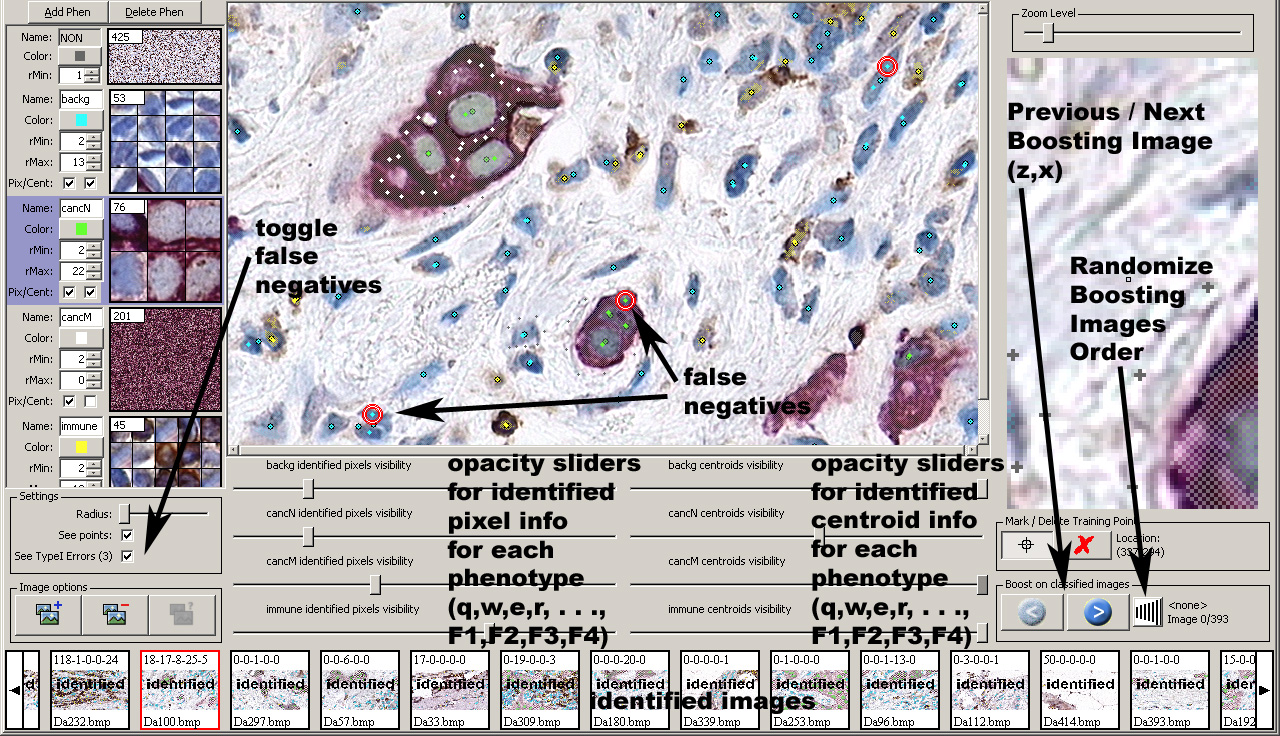
\includegraphics[width=476pt,height=281pt]{phenotyperetraining.jpg}
\label{fig:retraining}
\caption{\sf The anatomy of the retraining panel including the keyboard shortcuts for only those that are in addition to the {\sf phenotype training} panel. The image of the lymph node being retrained is from the Kohrt study\cite{kohrt}.}
\end{figure}

\subsection{Identified Image Display}

Those images classified will now have an updated thumbnail icon and display the text {\tt ``identified''} across their body. When these images are selected, the image is displayed normally, but now sliders for each phenotype will appear just below the image. The sliders on the left control the opacity of the pixels identified in that phenotype class and the sliders on the right control the opacity of the centroids identified in that phenotype class. If information is unavailable for whatever reason, the slider will be disabled. Function keys F1, F2, F3, F4 will set all sliders to an opacity of 0\%,33\%,66\%,100\% respectively.

\subsection{Viewing false negatives}

The checkbox ``See Type I Errors (e)'' (where ``e'' is the number of Type I errors in the current training image) will draw a red circle around each of the false negatives. This will aid retraining. If there are no type I errors, the checkbox will be disabled.

\subsection{Boosting the training set}

If the classification was performed with images in addition to those in the training set, the training set can be ``boosted'' to include more examples (see \cite{boosting} for more information about the usefulness of boosting). 

In the boosting panel, click the $\blacktriangleright$ button. An image not in the training set will be displayed on the screen. If an error was found, train over the error and this image will be automatically added to the training set and removed from the boosting set. The $\blacktriangleleft$ button will navigate backwards. The \framebox{\sf order / random} toggle button will order or randomize the image order in the boost set.

This is useful to ``beef up'' the training set to include more representative examples of the phenotypes precisely where {\bf GemIdent} is having trouble.

\subsection{Retraining advice for common situations}

Train over {\bf GemIdent}'s mistakenly classified pixels (Type II errors) using the ``NON'' phenotype. If {\bf GemIdent} was not able to identify some phenotype examples (Type I errors), train more examples using the respective phenotype.

\subsubsection{Persistent false negatives}

It is possible that all phenotypes of a class do not look the same. In fact, there may be multiple {\emph{subclasses}} of the phenotype. A subclass can appear relatively darker than the rest, lighter than rest, larger, smaller, etc. If {\bf GemIdent} is making many false negative mistakes, it may be because you have not trained for that particular subclass of the phenotype (see Fig. \ref{fig:subclasses}).

\begin{figure}[htp]
\centering
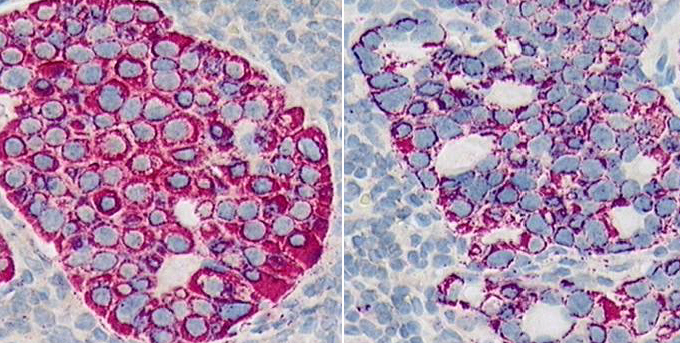
\includegraphics[width=300pt,height=153pt]{subclasses.jpg}
\label{fig:subclasses}
\caption{\sf Both images are from the same lymphnode from the Kohrt study\cite{kohrt}. The stained cells are cancer cells stained for AE1/3 with Fast Red red. Some regions of the tissue stain like the image on the left and other regions stain like the image on the left. These are two ``subclasses'' of the same phenotype (the left is named subclass ``A,'' the right, subclass ``B'').}
\end{figure}

If {\bf GemIdent} is having trouble with one of the subclasses it is most likely because it was neglected during training. Training for a particular phenotype must be diverse enough to cover the wide range of examples seen throughout the image set.

\subsubsection{Persistent misclassifications}

After retraining over mistaken regions multiple times, {\bf GemIdent} may still fail to correctly classify your phenotypes. This may be because the surrounding colors are too similiar to be teased apart (see Fig. \ref{fig:samecolors}). This is a limitation of the images themselves and not of the software. However, you may want to return to color training, remove your old colors, and train for new ones. Make sure the new colors are more specific. Train in the misclassified regions for more nuanced examples of the different shades. 

It may be helpful to even add new colors. For example, in Fig. \ref{fig:subclasses}, the nuclei in subclass ``B'' appear to have {\emph{purple}} membranes and the cells in subclass ``A'' appear to have {\emph{maroon}} membranes. If you have only trained for the maroon during color selection, {\bf GemIdent} will have difficulty classifying subclass ``B'' no matter the number of training points during phenotype training. Return to color selection and create a new color that represents the disenfranchised purple.

\begin{figure}[htp]
\centering
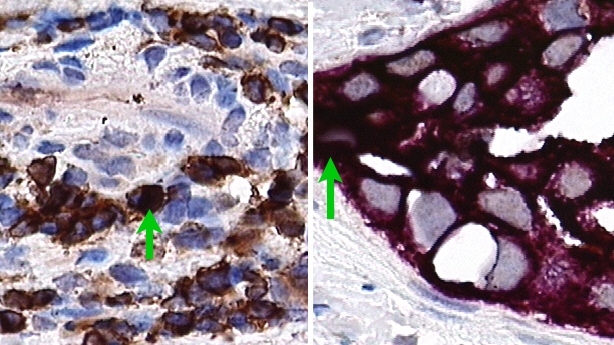
\includegraphics[width=300pt,height=178pt]{samecolors.jpg}
\label{fig:samecolors}
\caption{\sf The image on the left shows T-cells stained for CD4 with DAB brown. The arrow indicates a region of dark brown high stain intensity. The image on the right shows cancer cells stained for AE1/3 with Fast Red red. The arrow again indicates a region of dark red high stain intensity. The dark brown and dark red are the same color so {\bf GemIdent} may some have trouble telling the difference between T-cells and cancer cells}
\end{figure}

The more individual shade definitions, the more detailed information {\bf GemIdent} will have during classification, thereby the greater the accuracy.

\subsubsection{Problems with centroid locating}

{\bf GemIdent} may have trouble locating the centroids in classification blobs that are relatively small or large. Admittedly, the original centroid-finding algorithm is weak and we are seeking those with expertise to complement {\bf GemIdent} a more respectable algorithm (see section~\ref{open_source}).

That being said, there are still many things you can do to improve accuracy. 

If {\bf GemIdent} doesn't find centroids of small blobs, it is most likely because you did not train for enough small blobs. Retrain for more examples of this phenotype that are small and redo a classification and centers. If the objects of interest are themselves very small (less than 20 pixels total), noise presents a problem. You may want to artificially increase the number of pixels available by expanding the images using photo-manipulation software prior to loading them into {\bf GemIdent}.

Analagously, if {\bf GemIdent} places too many centroids inside large blobs, it is most likely because you did not train for enough large blobs. Retrain for more examples of this phenotype that are small and redo a classification and centers. Unfortunately, if the results are unsatisfactory after the mentioned exercise, then there is little you can do --- the basic centroid-finding algorithm is limited.

\subsection{Reclassification}

After the training images have been corrected and the set has been boosted, return to the {\sf classification} panel and redo the analysis. Please note that the machine learning classifiers will be rebuilt from scratch. All classifications are completely independent of each other.

After a few retrain-reclassification iterations, you may be confident enough to begin a full classification. The results will be more or less what you have observed in the training images. There is no recommended number of retrains, it depends on the application, what accuracy level is desired, and the classification parameters.

\section{Data Analysis}

After a successful classification, the data can be analyzed in the {\sf analysis} panel. This is only relevant for Bliss or NanoZoomer image sets where each classified image  is part of a larger global image.

\begin{figure}[htp]
\centering
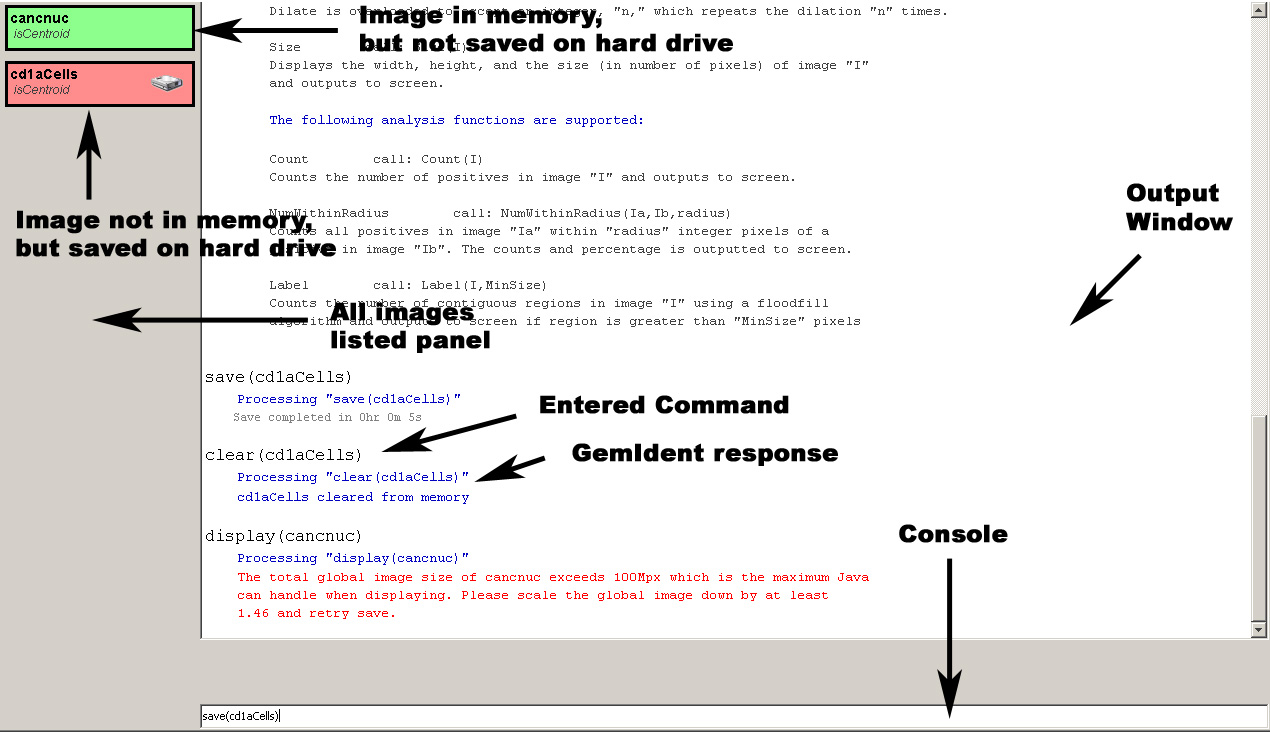
\includegraphics[width=476pt,height=281pt]{analysis.jpg}
\label{fig:analysis}
\caption{\sf The anatomy of the Data Analyis panel. There are no keyboard shortcuts. However, clicking on the image icons on the left panel will insert their names into the command line console.}
\end{figure}


\subsection{Using the interface}

Commands can be typed into the console and executed by pressing {\tt enter} much like any interpreted language. For a list of available functions, their descriptions, and their usage, and you may type {\tt help} at any time. Much like other interpreted languages, if you would like to access your previously entered commands, you can use the $\uparrow$ key on the keypad (as well as the $\downarrow$ key for the reverse direction).

As images are created, they will appear on the left panel as a rectangular subpanel that displays the name and the type. If the image is saved on the hard drive, a hard drive icon will appear inside. If the image is in memory its background will be green, if not, the background will be red.

Some functions take parameters that represent a distance or area. Pre-programmed into the analysis page is the conversion between the native unit (eg microns, feet, etc) and the pixel distances {\bf GemIdent} uses. Therefore, those parameters must be specified in the native unit, not in pixels.

\subsection{The system functions}

A ``system function'' does not take parameters.
Here are a list of the currently available functions. 
\subsubsection{\tt Build}

The first step after a fresh classification would be to build the global images from the classification results. Type {\tt build} into the console.

The global images have the same size as the entire scan and are represented as binary - white representing the presence of that phenotype and black representing its absence. Depending on the number of images in the set and your computer's capabilities, building times can vary. One global image will be built for every phenotype. 

You should see subpanels appear on the left panel bearing their names and their types (either ``isPixel'' for a phenotype whose pixels were identified or ``isCentroid'' for a phenotype whose centers were found). If you create a derivative of one of these core global images (e.g. scaling or dilating it), that derivative's type will be displayed as ``other.''

\subsubsection{\tt Clear}

By typing {\tt clear}, all images in memory will be flushed. This will delete an image permanently if it hasn't been stored to the hard drive.

\subsubsection{\tt SaveAll}

All images in memory will be saved to hard disk. All previously existing images on hard disk (with identical names) are {\emph{overwritten}}. To save individual images, use the {\tt Save} command.

\subsubsection{\tt LoadAll}

All images on hard disk are loaded into memory. All previously existing images in memory (with identical names) are {\emph{overwritten}}. To load individual images, use the {\tt Load} command.

\subsubsection{\tt Clean}

By typing {\tt clean} in the console, {\bf GemIdent} will now delete all the intermediate classification files as well as the color information files. This cannot be undone. If the globals have not been built yet, all the information that would be used to build them would be gone and the classification would have to be repeated. Additionally, you will no longer be able to retrain effectively because the masks are now deleted. 

This is useful to tidy up projects. During classification it is not uncommon for gigabytes of intermediate information to be stored that can be safely deleted {\emph{after}} the globals have been constructed and saved.

\subsubsection{\tt Mem}

At any time, you could type {\tt mem} in the console to get an idea on how much memory the {\emph{images}} use (not the entire program).

\subsubsection{\tt Thumb}

To a view the original scan (similiar to the helper in the color {\sf selection train} panel) type {\tt Thumb} at any time to spawn a new window displaying the global image.

\subsubsection{\tt Report}

It may be useful to have a report including a thumbnail image of the scan, counts \& error rates, and a transcript of the analyses you performed. A PDF can be auto-generated by typing {\tt Report} in the console. The file will be timestamped and placed in the output subdirectory. Additionally, it will auto-open in your operating system's PDF reader upon generation.

\subsubsection{\tt CorrectErrors}

Phenotype retraining gives the user limited ability to correct type II errors (false positives). The user must be allowed to ``review'' the entire global image and delete obvious errors. The optimal interface would be for the global image to display with the centroids overlaid. However, there are internal limits on the maximum image size. Using function {\tt CorrectErrors} will segment the global image and report back the number of segments (e.g. ``1,2, . . ., 7''). The segments can then be individually corrected (see the {\tt Correct} function).

\subsubsection{\tt Join}

The analysis page is multithreaded and can process any number of commands simultaneously using all available CPU's (compare to {\tt R}, {\tt Matlab}, or most other interpreted languages which can only process one command using one CPU at a time). You may wish for the computer to ``finish up'' all commands currently being processed before loading it with a new task. Calling {\tt Join} will delay the execution of new tasks until all previous executing tasks finish.

\subsection{Basic Image Operations}

\subsubsection{\tt Load, Save, Clear, \& Delete}

These basic operations are invoked using parentheses to specify it's target image (e.g. {\tt Delete(NewImage)}). Load will load the image into memory, Save will save it to the hard drive, Clear will flush it from memory, and Delete will clear it and delete the file on the hard drive (if it exists).

\subsubsection{\tt Display}

Java can display the target binary image in a new window. If the size exceeds your resolution, you are free to resize or scroll about in the image.

Java is practically limited in its display of images to images of size 100Mpx. If the image you are trying to display exceeds this size, you will obligated to scale it down by at least the factor specified in the error message.

\subsubsection{\tt Correct}

{\tt Correct} takes one integer as a parameter --- the correction segment you wish to correct (see ``CorrectErrors''). This will spawn a window displaying the image segment specified overlaid with the results for the phenotypes. You may scroll through the image and click on false positives. A red ``X'' will appear, crossing out each selection. At this point, that result is deleted from the respective global centroids image (be careful, each selection is permanent, an undo feature does not exist).

If you only wish to correct certain phenotypes, you can overload the {\tt Correct} function with those phenotypes.

\subsection{Binary Image Manipulations}

\subsubsection{\tt Erode}

This function will test every positive pixel in the image for four neighbors (North, South, East, and West neighbors). If the pixel lacks any of these neighbors it is erased, hence a ``N4 erosion.'' This would be useful to break apart blobs that exist in ``isPixel'' image types. Please note, by definition, if erode was performed on an ``isCentroid'' image, all data will be lost.

{\tt Erode} can be overloaded with an integer ``n.'' This will result in ``n'' consecutive erosions.

\subsubsection{\tt Dilate}

The opposite of Erode is Dilate. For every positive pixel, the four neighbors (North, South, East, and West neighbors) will be set positive. This is useful to merge blobs in ``isPixel'' images. Running a dilation on an ``isCentroid'' image will merely larger, diamond-shaped indications that a center is there. This may be useful to ``blow up'' a centroids image to the point where the centers are now the average size of the object.

{\tt Dilate} can be overloaded with an integer ``n.'' This will result in ``n'' consecutive dilations.

\subsubsection{\tt Or}

Or will combine the positives of two same-sized images together into a combined image. For each pixel in image A and image B, the output in the combined image will be the result of their non-exclusive or operation.

\subsubsection{\tt Scale}

Scale will change the size of the image using an inverse scale. For instance, if scale is run on image A with a scale parameter of 2, the resulting image will have half the width and half the height of image A (therefore a quarter of the total pixels). If a scale is run on image A with a scale parameter of 0.1, the resulting image will be ten times as wide and ten times as high (therefore 100 times more pixels). It is not uncommon when scaling in this direction to run out of memory. The error message will display the needed memory to perform the operation.

\subsubsection{\tt Size}

Use {\tt Size} to find the width, height, and total number of pixels in an image when considering it for display or scaling.

\subsubsection{\tt Count}

{\tt Count} will simply count the number of positive points in this image and display the result.

\subsection{Analysis Functions}

Analysis functions give the user the ability to discover spatial and geometric relationships between the phenotypes. {\bf GemIdent} was designed for the user to get more information than just merely the counts. This is where the magic of knowledge discovery takes place. A transcript of all analysis calls will be appended in auto-generated reports (see ``report'' in system functions).

\subsubsection{\tt NumWithinRadius}

An interesting question may be to ask ``how many of phenotype A are within r units of phenotype B.'' Calling {\tt NumWithinRadius(PhenA,PhenB,r)} will yield the total counts of Phenotype A, the subcount of those within r units of a positive Phenotype B, and the percentage.

\subsubsection{\tt NumWithinRing}

The same as {\tt NumWithinRadius} except you may specify a minimum radius and maximum radius.

\subsubsection{\tt DistanceAwayDistr}

Extending {\tt NumWithinRadius} it may be interesting to look at the {\emph{distribution}} of distances between Phenotype A and Phenotype B. {\tt DistanceAwayDistr} will tabulate these distances and display them in a auto-sized histogram and auto-generate a CSV file.

\subsubsection{\tt Label}

For images of type ``isPixel'' where maybe entire contiguous regions are identified, it may be useful to know how many separate regions exist. {\bf GemIdent} will use a floodfill algorithm\cite{floodfill} and return the centers and the size of the individual blobs. The ``MinSize'' parameter filters all noise below a certain number of units$^2$ (you don't want every individual noise pixel to be counted as a separate blob). {\tt Label} will display the blob size and the location of the center as well as auto-generate a CSV file.

\subsubsection{\tt DataDump}

The centroid information can be dumped to a CSV file for analysis outside of {\bf GemIdent}. Calling {\tt DataDump(PhenA,PhenB,$\ldots$)} will create a text file with the header \\ {\tt ``PhenA\_x,PhenA\_y,PhenB\_x,PhenB\_y,$\ldots$}
 and each line would describe one centroid in each of the phenotypes.

\subsection{Scripting}

If there are repeated complicated analyses that you wish to do, it may be more convenient to create a script file. {\bf GemIdent} accepts text files (in {\tt txt} format) where each line is one command. To run a script file select the {\sf Load and Run Analysis Script . . .} menu item in the {\sf Script} menu.

Be careful to place {\tt Join}'s in proper places otherwise all commands will execute simultaneously.

\begin{figure}[htp]
\centering
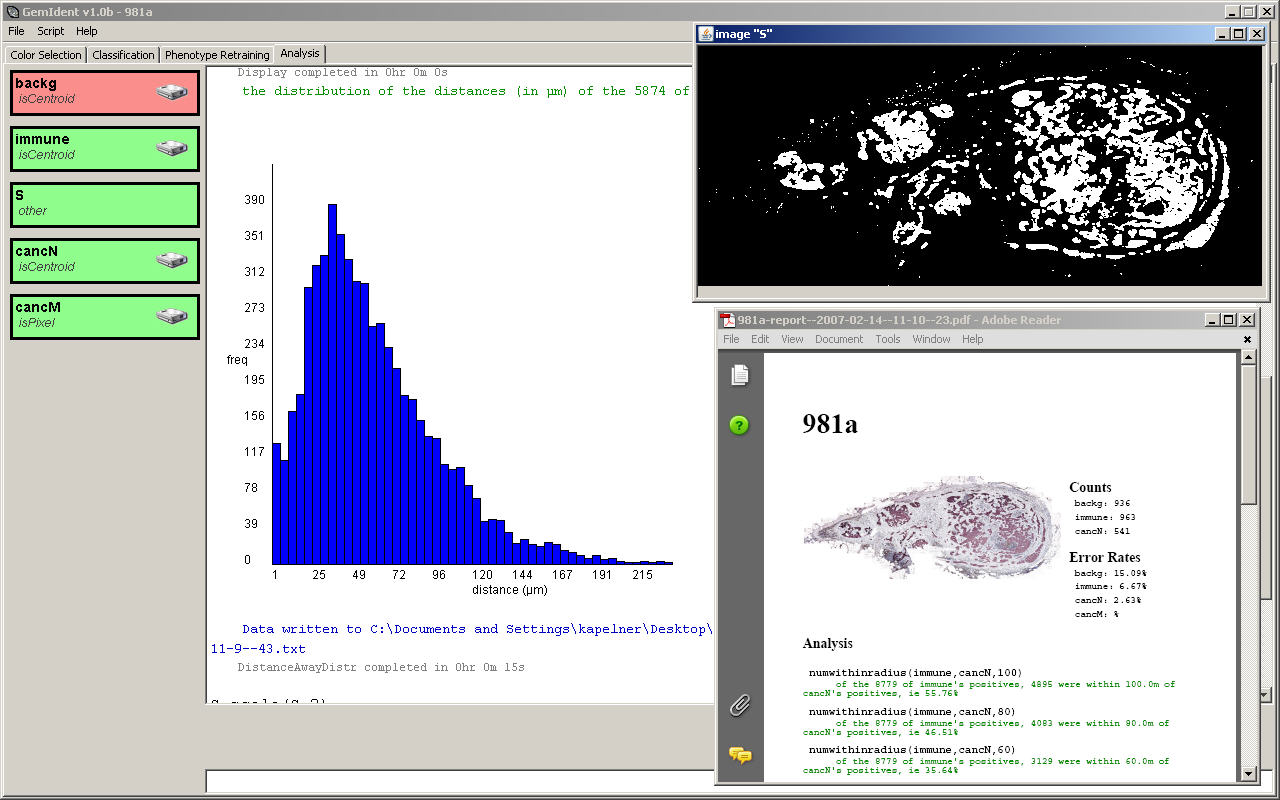
\includegraphics[width=7in, height=4.375in]{analysisdata.jpg}
\caption{\sf An example of the command-line data analysis panel in action analyzing results of a classification of a lymph node from the Kohrt study\cite{kohrt}. The histogram (generated via the {\tt DistanceAwayDistr} function) displays the distribution of distances from T-cells to neighboring cancer cells. The binary image of cancer membrane (displayed using the {\tt Display} function) is the result of an pixel-only classification. The open PDF document is the autogenerated report of the analysis (using the {\tt Report} function) which includes a thumbnail view of the entire lymphnode, counts and Type I error rates for all phenotypes, as well as a transcript of the analyses performed.}
\label{fig:DataAnalysisInAction}
\end{figure}

\section{Known Bugs}

The following are known bugs in {\bf GemIdent}:

\begin{itemize}
\item There seems to be a small memory leak during classification. This is only a problem when hundreds to thousands of images are classified in one run. A workaround is to close the program upon completion of classification, and reopen.
\item During classification pre-processing, the program may hang indefinitely during the ``classifier generation'' step. In order to recover, press the \framebox{\sf Stop} button and then restart the classification.
\item The scrollbar for the pane that houses the stain / phenotype info viewers sometimes does not allow all the viewers to be seen. Behavior varies from platform to platform.
\end{itemize}

\section{Open-Source information\label{open_source}}

{\bf GemIdent} was developed purely in Java 6 (see {\tt www.sun.com/java}). The code has been open-sourced under GPL2 and is located on github at \url{https://github.com/kapelner/GemIdent}.

\subsection*{Dependencies}

{\bf GemIdent} leverages many open-source libraries:
\begin{description}
\item[JAMA] --- Java Matrix Package (see http://math.nist.gov/javanumerics/jama/). This libary supports matrix multiplication in order to compute color training information
\item[COLT] --- CERN's libraries for technical and scientific computing (see http://dsd.lbl.gov/~hoschek/colt/). The ``BitMatrix'' and ``BitVector'' libraries were altered to provide a data structure for storing classification results
\item[iText] --- the free Java PDF library (see http://www.lowagie.com/iText/). This provides support for exporting PDF's using the {\tt Report} function.
\end{description}

\section{Glossary}
\begin{description}
\item[A panel] - is a portion of {\bf GemIdent} that serves a particular function: color training, phenotype training / retraining, classification, and analysis. Panels can be accessed by clicking the appropriate tab on the top of the program window.
\item[A blob] - is an abbreviation that designates a contiguous region of the same phenotype.
\item[A centroid] - is the center of a classified object most often calculated by taking the average of the points in the identified blob.
\item[Statistical Machine Learning] - designates an algorithm which takes two types of data: training data which are multivariate observations for which the labels are known and anonymous data that need to be identified or labelled. The training data serve to determine good discriminatory features and establish a classification rule which takes the multivariate data from the anonymous set and returns a class prediction, the program's best guess of the phenotype. A good reference to consult is the book on Statistical Learning by Hastie et al, 2001\cite{hastie}.
\item[Boosting] - Boosting is an iterative procedure for improving a learning algorithm, 
by incrementally adding to the current learned function. 
At every stage, more data are added to help the program correct its weakness, in the classical framework
this is often done automatically by using a weak learning algorithm, in this implementation,
the user specifies the improvements to make, adding more data of the type that
are not correctly identified.
\item[Classification] - given a pixel in an image, {\bf GemIdent} will predict which phenotype it's most similiar to. If it's not similiar to any, it will be marked as ``NON'' and will be invisible in the retraining panel.
\item[Random Forest] - a machine learning classifier developed by \cite{breiman} 
that creates a collection of specialized decision trees. The trees vote on the incoming data and the majority vote wins.
\item[Decision Tree] - a tree structure that partitions the data successively
 into subsets as homogeneous as possible
with regards to the labels the program is trying to explain.
An early implementation that was particularly successful and was an ancestor
to the random forests is called CART (Classification and Regression Tree)\cite{cart}.
\item[Mahalonobis distance] - is a special distance used in statistics
that accounts for correlations between the variables used as coordinates and their varying variances.
It is a weighted Euclidean distance that renormalizes the variables in different groups, and is the basis of Fisher's linear discriminant analysis which was one of the first classification algorithms\cite{mahalanobis}.
\item[Type I errors (false negatives)] - designate points where the user trained for a certain phenotype, but {\bf GemIdent} failed to find it. 
\item[Type II errors (false positives or misclassifications)] - points that {\bf GemIdent} identified, but are either not representative of a phenotype at all or not actually the phenotype sought.
\end{description}

%\clearpage

\begin{thebibliography}{10}

\providecommand{\url}[1]{#1}
\csname url@samestyle\endcsname
\providecommand{\newblock}{\relax}
\providecommand{\bibinfo}[2]{#2}
\providecommand{\BIBentrySTDinterwordspacing}{\spaceskip=0pt\relax}
\providecommand{\BIBentryALTinterwordstretchfactor}{4}
\providecommand{\BIBentryALTinterwordspacing}{\spaceskip=\fontdimen2\font plus
\BIBentryALTinterwordstretchfactor\fontdimen3\font minus
  \fontdimen4\font\relax}
\providecommand{\BIBforeignlanguage}[2]{{%
\expandafter\ifx\csname l@#1\endcsname\relax
\typeout{** WARNING: IEEEtran.bst: No hyphenation pattern has been}%
\typeout{** loaded for the language `#1'. Using the pattern for}%
\typeout{** the default language instead.}%
\else
\language=\csname l@#1\endcsname
\fi
#2}}
\providecommand{\BIBdecl}{\relax}
\BIBdecl

\bibitem{kohrt}
H.~E. Kohrt, N.~Nouri, K.~Nowels, D.~Johnson, S.~Holmes, and P.~P. Lee,
  ``Profile of immune cells in axillary lymph nodes predicts disease-free
  survival in breast cancer,'' \emph{PLoS Med}, vol. 2(9), p. e284, 2005.


\bibitem{boosting}
Y.~Freund and R.~Schapire, ``A decision-theoretic generalization of on-line
  learning and an application to boosting,'' \emph{Journal of Computer and
  System Sciences}, vol.~55, no.~1, 1997.


\bibitem{breiman}
\BIBentryALTinterwordspacing
L.~Breiman, ``Random forests,'' \emph{Machine Learning}, vol.~45, no.~1, pp.
  5--32, 2001. [Online]. Available:
  \url{citeseer.ist.psu.edu/breiman01random.html}
\BIBentrySTDinterwordspacing


\bibitem{cart}
L.~Breiman, L.~Friedman, R.~Olshen, and C.~Stone.
\newblock {\em Classification and Regression Trees}.
\newblock Wadsworth and Brooks, 1984.



\bibitem{hastie}
R.~Tibshirani, T.~Hastie and J.~Friedman, \emph{The Elements of Statistical
  Learning}.\hskip 1em plus 0.5em minus 0.4em\relax NY.: Springer, 2001.


\bibitem{floodfill}
``\url{http://en.wikipedia.org/wiki/Flood\_fill}.''

\bibitem{mahalanobis}
P.~C.~ Mahalanobis, On the generalised distance in statistics, 
\emph{Proceedings of the National Institute of Science of India}, 
vol 12, p49-55, 1936.

\end{thebibliography}

\end{document}
